\documentclass[12pt,a4paper]{report}

\usepackage[utf8]{inputenc}
\usepackage[T1]{fontenc}
\usepackage{lmodern}
\usepackage{titlesec} 
\usepackage{graphicx}
\usepackage{microtype}
\usepackage{hyperref} 
\usepackage{amssymb}
\usepackage[frenchb]{babel}
\usepackage{listings}
\usepackage{amsmath}
\usepackage{enumitem}
\usepackage{float} 
\usepackage{fancyhdr}
\usepackage{multirow}

\usepackage{pict2e}

\usepackage{listings}	  

\lstdefinestyle{customstyle}{
    basicstyle=\footnotesize,
    breakatwhitespace=false,         
    breaklines=true,                 
    captionpos=b,                    
    keepspaces=true,                                                                                       
    tabsize=4,
    frame=single,
    moredelim=[is][\underbar]{_}{_}
}
\lstset{style=customstyle}

\title{\textsc{Modélisation et analyse des systèmes logiciels hétérogènes}\vspace{0.5cm}\\\large{\textit{Rapport du Module d'initiation à la recherche}}}
\author{Antoine Forgerou \and Jérémy Bardon \and Nicolas Bourdin}
\date{}

\fancypagestyle{empty}{
  \fancyhead[L]{	
\includegraphics[scale=0.5]{ressources/logoUniv.jpg}}
  \fancyhead[R]{Master Informatique\\2014/2015}
  \fancyfoot[L]{Responsable : M$^r$ Christian Attiogbé\\Équipe AeLoS}
  \fancyfoot[R]{Version du \today}
}

% Permet de masquer les affichages de "Chapitre" 
\titleformat{\chapter}[hang]{\bf\huge}{\thechapter}{2pc}{} 
\begin{document}
	\renewcommand{\contentsname}{Sommaire}
	\pagenumbering{gobble}

	\maketitle	

\chapter*{Remerciements}
Ce stage au sein de l'équipe de recherche AeLoS nous as donné
l'opportunité d'avoir un aperçu du monde de la recherche. 
\\\\
C'est pourquoi nous tenons à remercier M$^r$ Christian Attiogbé 
ainsi que l'équipe AeLoS pour nous avoir permis d'apporter notre
contribution à l'un de leurs sujets de recherche.

\newpage

	\tableofcontents	
	\newpage

	\setlength{\unitlength}{1cm}
	\setcounter{page}{1}
	\pagenumbering{arabic}
\nocite{*}
\chapter{Introduction}
Ce document est un rapport rassemblant le travail que nous avons effectué dans le cadre du module 
d'initiation à la recherche au sein du Master 1 ALMA. Ce module permet d'initier 
les étudiants au travail de recherche en informatique, en immersion dans une équipe
du laboratoire LINA. 
\\\\
Le sujet de recherche auquel nous avons contribué est le suivant : 

\begin{center}
	  \textbf{Modélisation et analyse des systèmes logiciels hétérogènes}
\end{center}

La préoccupation de l'équipe qui nous a accueilli est de trouver un moyen d'assurer la cohésion 
de modèles d'un système
hétérogène lors d'opérations d'ajout et/ou de suppression des modèles le composant. 
Tous les modèles seront alors capables de communiquer ensemble; et dans un premier temps, 
le choix a été fait de s'appuyer sur l'exemple d'automates que l'on voudrait composer.
\\\\
Au cours de ce rapport, différents points seront abordés. Tout d'abord une 
présentation du laboratoire LINA ainsi que de l'équipe AeLoS que nous avons intégrée le 
temps du module de recherche. Nous reviendrons alors plus en détail sur la 
problématique soulevée par le sujet pour ensuite présenter les 3 solutions proposées
par l'équipe. Ensuite, nous expliquerons la solution que nous avons choisie de mettre 
en place et nous rentrerons au cœur du projet avec la présentation de la solution
que nous avons implémentée.	

\chapter{Présentation du laboratoire}
Acteur central du développement de l'informatique dans la région des Pays de La Loire, le LINA (Laboratoire d'Informatique de Nantes Atlantique) est un laboratoire de recherche en sciences et technologies du logiciel qui est dirigé par Pierre Cointe. Avec ses 180 membres, ce laboratoire est actuellement situé sur deux sites Nantais : la Lombarderie (Faculté des Sciences et Techniques) et la Chantrerie (Ecole des Mines et Polytech' Nantes).


\section{Les différentes équipes}
Le LINA est composé des équipes suivantes : 
\begin{itemize}
  \item AeLoS : \textbf{A}rchitectures et \textbf{Lo}giciels \textbf{S}ûrs
  \item ASCOLA : \textbf{AS}pect and \textbf{CO}mposition \textbf{LA}nguages
  \item AtlanMod : \textbf{Atlan}tic \textbf{Mod}eling 
  \item ComBi : \textbf{Com}binatoire et \textbf{Bi}oinformatique
  \item DUKe : \textbf{D}ata \textbf{U}ser \textbf{K}nowledg\textbf{e}
  \item GDD : \textbf{G}estion de \textbf{D}onnées \textbf{D}istribuées
  \item OPTI : Optimisation globale, optimisation multi-objectifs
  \item TALN : \textbf{T}raitement \textbf{A}utomatique du \textbf{L}angage \textbf{N}aturel
  \item TASC : Programmation par contraintes
\end{itemize}

\chapter{L'équipe AeLoS}	

L'équipe Architectures et Logiciels Sûrs (AeLoS), est dirigée par Christian ATTIOGBE.

Le projet central de cette équipe s'appuie sur les trois thématiques suivantes :
\begin{itemize}[label=$\circ$]
  \item \textbf{Architecture} qui couvre une approche descendante du logiciel,
  \item \textbf{Composants logiciels corrects} couvre l'approche ascendante du logiciel,
  \item \textbf{Multiformalisme et analyse multifacette} qui s'attaque au défi d'interopérabilité et de l'analyse globale du logiciel.
\end{itemize}

\section{Les membres}
Une récente liste des membres est disponible sur le site du LINA, à l'adresse suivante : \\
\url{http://www.lina.univ-nantes.fr/spip.php?page=membres&id_equipe=15&lang=fr}

\chapter{Présentation du sujet de recherche}
\section{Problématique}

La construction rigoureuse d'un logiciel se fait à partir de son modèle. Pour des 
logiciels complexes (par exemple ceux qui ont de nombreux composants différents -- 
hétérogènes-- et qui communiquent), on dispose de plusieurs modèles (hétérogènes 
aussi) qui doivent interagir de façon cohérente, pour garantir l'interopérabilité 
sémantique entre les modèles puis les composants logiciels. Le domaine des systèmes 
embarqués (et aussi des objets connectés) regorge d'exemples.\\

\subparagraph*{Prenons un exemple concret :\\ }
un système de surveillance filme et transmet des images sur un moniteur distant comme ceci : 

\begin{figure}[h]
	\centering
	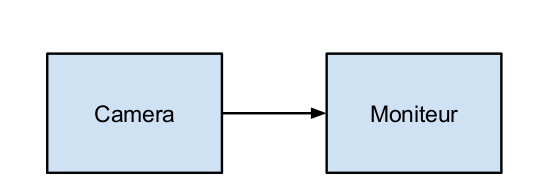
\includegraphics[scale=0.5]{ressources/camera-moniteur.png}
	\caption{Exemple n1 - Camera Moniteur}
\end{figure}
%Integrer image : automate camera + automate moniteur
Que se passerait il si l'on souhaite alors sauvegarder les vidéos de surveillance sur une base de données comme ci-dessous?
Notre rôle est de faire en sorte que les différents modèles qui composent le système fonctionnent correctement malgré l'ajout de nouveaux composants. \\\\
\begin{figure}[!h]
	\centering
	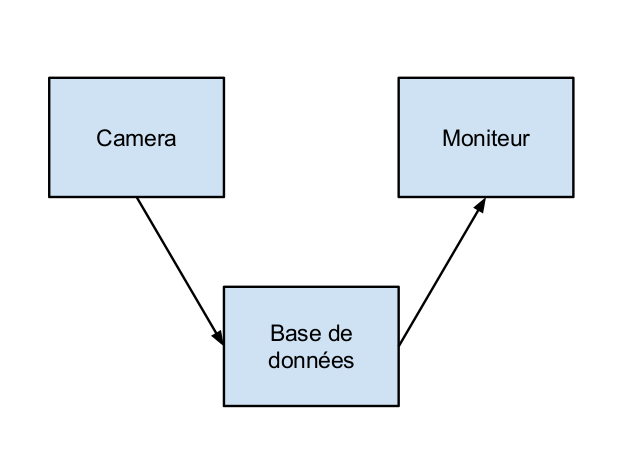
\includegraphics[scale=0.5]{ressources/camera-bdd-moniteur.png}
	\caption{Exemple n2 - Camera BDD  Moniteur}
\end{figure}


\paragraph*{Autre exemple :\\}

Un logiciel comme YMPD\footnote{\href{http://www.ympd.org}{ympd.org}} permettant la lecture côté serveur de piste audio, est constitué de deux langages que tout oppose : \begin{itemize}
  \item Le langage C (de bas niveau)
  \item Le langage Javascript (de très haut niveau)
\end{itemize}
Cependant, le logiciel doit fonctionner correctement malgré l'utilisation de ces langages différents. 
Ainsi, l'utilisation de modèles rend possible la représentation de systèmes et permet 
le fonctionnement du logiciel dans un langage commun qui n'est autre que le modèle d'automate.
D'où la nécessite de manipuler les modèles.


\section{Solutions proposées par l'équipe AeLoS}\label{sec:Solutions}
Pour répondre à la problématique, l'équipe AeLoS nous a proposé 3 façons de 
faire tout en nous laissant la liberté d'en proposer d'autres.
Dans le but de simplifier les exemples, nous avons fait le choix de représenter 
les modèles comme des formes géométriques que l'on essayerait d'emboîter.
\\\\
La première solution consiste à adapter un des modèles au deuxième quand cela 
est possible. On peut prendre l'exemple du théorème de Kleene qui assure qu'un 
automate à états finis peut être écrit sous la forme d'une expression 
rationnelle et vice et versa. Par conséquent on peu adapter des composants
ayant comme modèle les automates ou les expressions régulières.

\begin{figure}[h]
	\centering
	
\includegraphics[scale=1]{ressources/solution1.png}
	\caption{Solution 1 - Adaptation d'un modèle}
\end{figure}

Dans cet exemple c'est le composant de gauche qui s'est adapté -- par une 
légère modification -- pour pouvoir interagir avec la partie droite.

\newpage
L'approche qui parait la plus évidente mais qui peut se révéler complexe 
consiste à intégrer un troisième modèle dans le système. Ce dernier va alors 
jouer le rôle de passerelle entre les deux modèles que l'on veut faire 
communiquer.

\begin{figure}[h]
	\centering
	
\includegraphics[scale=1]{ressources/solution2.png}
	\caption{Solution 2 - Interface entre les modèles}
\end{figure}
 
Le principe est de faire interagir les modèles ensemble puis d'effectuer des 
vérifications pour déterminer si les modèles peuvent communiquer à 100\%, 
en partie ou pas du tout. Cela rentre dans une approche globale (Plug'N'check) 
que l'équipe étudie.

\begin{figure}[h]
	\centering
	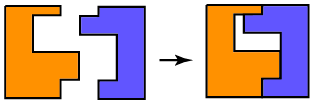
\includegraphics[scale=1]{ressources/solution3.png}
	\caption{Solution 3 - Plug'N'Check}
\end{figure}

L'exemple montre que certaines parties sont satisfaites mais d'autres parties ne 
peuvent pas communiquer.
\\\\
Dans le cadre de notre stage d'initiation à la recherche, nous nous sommes 
orientés vers la première solution. Nous avons donc entrepris de transformer 
des modèles dans un langage commun afin de permettre de les 
interfacer.
\\\\
Il est admis que les automates sont une spécialisation de graphe, ce qui 
signifie que n'importe quel automate peut-être représenté sous forme de graphe. 
C'est la raison qui nous a poussé à utiliser le langage \emph{DOT} dans le projet.

\newpage
\section{Rappel sur les Automates}

    Les automates sur lesquels nous nous appuierons pour ce projet sont les automates à états fini, 
    non-déterministes contenant des $\epsilon$-transitions.\\
    
    Rappelons la définition de l’automate à états fini non déterministe :
\begin{enumerate}
    \item un ensemble fini d’états, souvent noté Q 
    \item un ensemble fini de symboles, appelé alphabet et souvent noté $\Sigma$ 
    \item une fonction de transition, souvent nommée $\delta$, qui reçoit comme arguments un état de Q et un symbole de $\Sigma$ ou la chaîne vide notée $\epsilon$ et qui rend comme résultat une partie de Q \begin{center}$\delta : Q * ( \Sigma \cup \epsilon ) \rightarrow P(Q)$ \end{center}
    \item un état initial q0, appartenant à Q
    \item un sous-ensemble F de Q constitué des états finals, ou états acceptants.\\
\end{enumerate}    

    Voici un exemple d'automate, extrait de notre projet :\\

\begin{figure}[h]
	\centering
	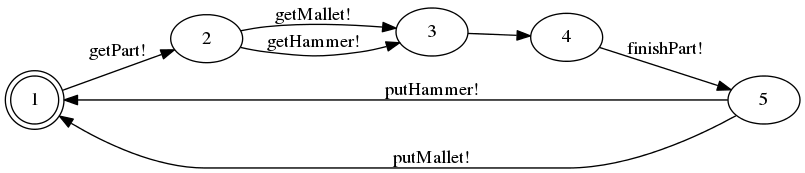
\includegraphics[scale=0.5]{ressources/img.png}
	\caption{Automate du "jobber" qui usine des pièces}
\end{figure}
  
    En appliquant la définition donnée ci-dessus, on obtient pour notre exemple :
\begin{enumerate}
  \item l'ensemble d'états Q = \{1,2,3,4,5\}
  \item l'alphabet $\Sigma$ = \{getPart!,finishPart!,getMallet!,putMallet!,getHammer!,putHammer!\}
  \item l'état initial q0 = 1 et il n'y a pas d'état final F = \{\}
  \item la liste des fonctions de transition : 
  \begin{enumerate}
    \item $\delta$(1,getPart!) = 2 
    \item $\delta$(2,getHammer!) = 3 et $\delta$(2,getMallet!) = 3 
    \item $\delta$(3,$\epsilon$) = 4 
    \item $\delta$(4,finishPart!) = 5 
    \item $\delta$(5,putMallet!) = 1 et $\delta$(5,putHammer!) = 1 
  \end{enumerate}
\end{enumerate}

\section{UPPAAL : un outil de modélisation des automates}
\textsc{Uppaal} est un environnement intégré d'outils pour la modélisation , la validation et la vérification des systèmes temps réel modélisés comme des réseaux d' automates.
\\\\
\textsc{Uppaal} se compose de trois parties principales: 
\begin{itemize}[label=$\circ$]
  \item{un langage de description,}
  \item{un simulateur,}
  \item{un vérificateur de modèle.}
\end{itemize} 

  Le langage de description est un langage de commande non-déterministe avec des   
  types de données (par exemple des entiers, des tableaux, etc.) . Il se sert de la 
  modélisation ou du langage de conception pour décrire le comportement du système 
  grâce à des réseaux d'automates étendus avec des variables d'horloge et des données.\\ 

  Le simulateur est un outil de validation qui permet l'examen de possibles 
  exécutions d'un système au début de la conception(ou la modélisation) et fournit 
  un moyen peu coûteux de détection de défaut avant la vérification par le vérificateur 
  de modèle qui couvre l'ensemble des comportement dynamique du système.\\

  Le modèle peut vérifier les propriétés invariantes et l'accessibilité 
  en explorant l'espace et l'état d'un système, c'est à dire l'analyse de l'accessibilité 
  en termes d'états symboliques représentés par des contraintes.

\section{Le format DOT}

  Le langage DOT est un langage de description de graphe dans un format texte. C'est une manière simple de décrire des graphiques que les humains et les programmes informatiques peuvent utiliser. Les graphes DOT sont généralement des fichiers avec pour extension un .gv (ou .dot).\\

  La syntaxe DOT peut aussi bien décrire des graphes non-orientés que des graphes orientés, comme des automates finis.
  Il est possible de placer des étiquettes sur les transitions pour par exemple leurs donner un nom ou une explication. Le langage possède aussi des attributs permettant une description graphique plus poussée, par exemple choisir la couleur d'un nœud ou de dessiner une transition en pointillé.

\subsection{Graphe non-orienté}

\begin{lstlisting}[caption=Description textuelle en DOT]
graph monGraphe {
    a -- b -- c;
    b -- d;
}
\end{lstlisting}

\begin{figure}[!h]
  \centering
  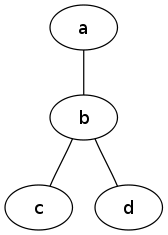
\includegraphics[scale=0.3]{ressources/grapheNO.png}
  \caption{Résultat de visualisation}
\end{figure}

\subsection{Graphe orienté}

\begin{lstlisting}[caption=Description textuelle en DOT]
graph monGraphe {
    a -> b -> c;
    b -> d;
}
\end{lstlisting}

\begin{figure}[!h]
  \centering
  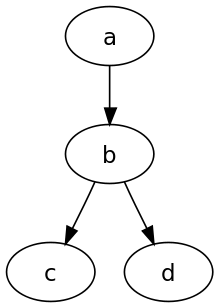
\includegraphics[scale=0.3]{ressources/grapheO.png}
  \caption{Résultat de visualisation}
\end{figure}

\chapter{Gestion du projet}
\section{Contexte de travail}
Nous sommes une équipe de 3 étudiants qui avons participé
 au sujet de recherche 
"\emph{Modélisation et analyse des systèmes logiciels hétérogènes}" mené par 
M$^r$ Christian Attiogbé, directeur de l'équipe de recherche AeLoS.
\\\\
Notre participation au projet s'inscrit dans 
le cadre de l'UE\footnote{UE: Unité d'enseignement} Initiation à 
la recherche et nous avions donc la matinée du mercredi pour effectuer
des réunions hebdomadaires et avancer sur le projet en équipe qui 
a débuté au mois de janvier pour finir au mois d'avril (le 28, jour de la soutenance).

\section{Déroulement dans le temps}
Afin de gérer l'avancée du projet et la répartition des tâches nous avons utilisé
un diagramme de Gantt. Celui-ci nous as permis de nous fixer des objectifs à atteindre
et de pouvoir prévoir à l'avance ce que l'on pourrait faire.
\\\\
Les tâches du projet se sont découpés en 2 grandes parties : la rédaction du rapport
et l'implémentation sachant que nous avons fait un travail préliminaire pour
comprendre et nous approprier le sujet.

\begin{figure}[H]
  \centering
  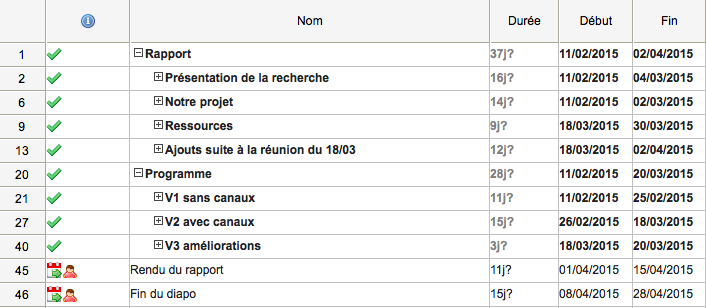
\includegraphics[scale=0.6]{ressources/taches.png}
  \caption{Tableau résumé des tâches}
\end{figure}

On peut remarquer que la rédaction du rapport est découpée dans le temps, ce qui 
signifie que l'on a commencé avec les éléments que nous avions au fur et à mesure: 
la présentation du laboratoire pour commencer puis des ajouts et des ajustements vers la fin.
\\\\
En parallèle, l'implémentation de notre module est divisée en \emph{versions} que nous
avons établis. En effet, chacune d'entre elles correspondent à une étape (un lot de fonctionnalités)
que nous voulions avoir une fois la version finie.

\begin{figure}[!h]
  \centering
  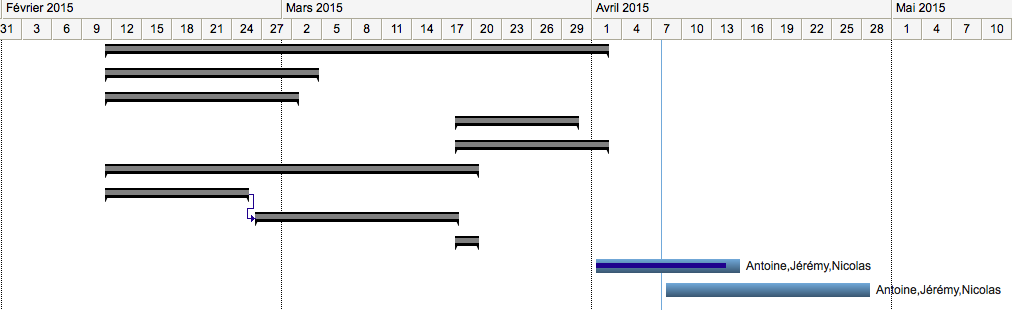
\includegraphics[scale=0.4]{ressources/gantt.png}
  \caption{Diagramme de Gantt}
\end{figure}

La partie supérieure du diagramme correspond à la rédaction du rapport
tandis que la partie inférieure suit l'avancement de l'implémentation.
\\\\
En analysant ce diagramme on peut comprendre que la rédaction du rapport a été
une préoccupation majeure car il s'agit du compte-rendu qui pourra permettre 
à l'équipe AeLoS de reprendre notre travail. En effet, sa rédaction a commencé dès
le départ et a même continuer après que la version 3 de l'implémentation soit terminée.
\\\\
Il est aussi possible de voir que nous avons -- vers le milieu du mois de mars -- concentrer
nos effort sur l'implémentation afin d'avoir des résultats. Une fois cette version intermédiaire
terminée nous avons pu continuer la rédaction du rapport en parallèle avant de 
finaliser celui-ci par plusieurs corrections -- de M$^r$ Attiogbé -- pour ensuite passer à l'élaboration 
d'une présentation pour la soutenance.


\newpage
\chapter[Hetersys : notre solution]{Hetersys\footnote{Heterogeneous systems: Tiré du nom du sujet de recherche "Modélisation et analyse des systèmes logiciels hétérogènes"} : notre solution}
\section{Introduction}

Notre but est de pouvoir composer n'importe quel type d'automate en utilisant 
\textsc{Uppaal}. Celui-ci propose de créer des automates et de les rassembler sous forme de projets 
mais il faut obligatoirement dessiner ces automates avec les outils mis à disposition
par \textsc{Uppaal}.
\\\\
Etant donné que les automates sont un sous-ensemble des graphes, notre module propose 
d'importer directement un automate -- décrit sous forme de graphe -- dans un projet 
\textsc{Uppaal} pré-existant. 

\begin{figure}[h]
  \centering
  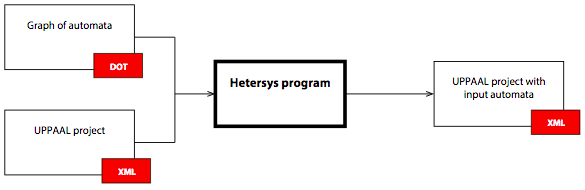
\includegraphics[scale=0.3]{ressources/ProgramScheme.png}
  \caption{Entrées et sorties du programme}
\end{figure}

Pour la description du graphe, nous avons choisi de nous appuyer
sur le format DOT bien connu qui est selon nous un langage très simple et minimaliste 
qui permet de construire des graphes très rapidement.

\section{Conception}

Comme évoqué dans l'introduction, la fonctionnalité attendue de notre module 
est de pouvoir intégrer un automate dans un système déjà composé de plusieurs
automates. 
\\\\
Dans un premier temps nous avons fait le choix d'utiliser le format DOT pour 
la description des automates -- sous forme de graphe -- et le logiciel \textsc{Uppaal}
qui permet de faire de la composition d'automates.
\\\\
Afin d'assurer l'extensibilité de notre module, nous n'avons pas tout simplement
converti le format DOT en format \textsc{Uppaal}. En effet, l'automate en entrée
est transposé sous forme de graphe -- en mémoire -- par un \emph{importeur} qui 
le donne ensuite à un \emph{exporteur} s'occupant de la conversion.

\begin{figure}[H]
  \centering
  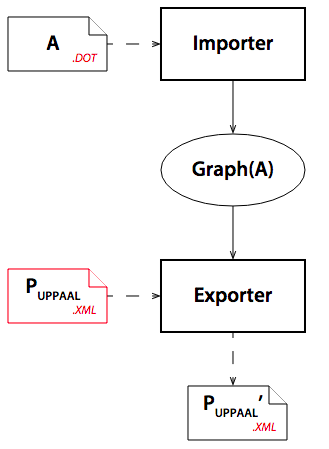
\includegraphics[scale=0.6]{ressources/archi2.png}
  \caption{Composants du logiciel}
\end{figure}

Ce type de fonctionnement permet facilement d'intervertir les modules
importeur et exporteur ainsi que d'ajouter facilement de nouveaux formats d'entrée
et/ou de sortie.
Quelque soit le format utilisé pour définir l'automate en entrée et le système,
le fonctionnement reste identique car le but est d'ajouter l'automate dans le
système. 

\begin{equation}
P_{UPPAAL}' = P_{UPPAAL} + XML(Graph(A))
\end{equation}
\\\\
Ce module constitue un noyau d'application mais pour les besoins de la
recherche il évoluera pour aussi permettre la suppression d'un automate dans le système.
\\\\
Le but du sujet de recherche étant d'assurer la cohésion entre les modèles 
d'un système hétérogène, le module assure un certain nombre de vérifications (voir \ref{ssec:VerifList})
avant d'effectuer l'action demandée. 
\\\\
Pour des vérifications plus poussées, ìl
faut aussi importer les automates du système dans le module et 
on va alors utiliser un second \emph{importeur} qui connait le format des automates
dans le système (XML pour \textsc{Uppaal}).

\section{Architecture logicielle}

L'architecture interne du programme a été pensée pour être la plus modulaire possible 
ce qui signifie que l'on peut facilement importer et/ou exporter dans un autre format
sans changer ce qui existe déjà. 
\\\\
En effet, le programme possède une représentation interne de l'automate sous forme 
de graphe ce qui rend ce genres d'ajustements plus simples. Les parties \emph{importer}
et \emph{exporter} constituent donc les points d'extension de notre programme.

\begin{figure}[H]
  \centering
  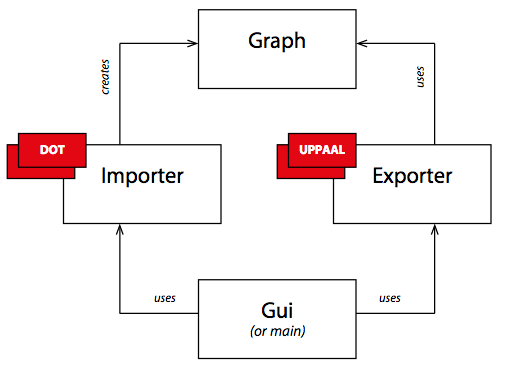
\includegraphics[scale=0.6]{ressources/archi.png}
  \caption{Composants du logiciel}
\end{figure}

Nous avons mis à disposition une interface graphique mais nous l'avons conçue dans l'optique 
de la découplée le plus possible du moteur de l'application. Il serait alors aisé de la supprimer
ou de la remplacer puisqu'elle suit le patron de conception MVC. 
\\\\
Par conséquent, la routine principale du programme se trouve au niveau du 
\emph{modèle} qui se charge de dérouler le programme tout en interagissant 
avec l'interface.

\section{Fonctionnement interne}

La partie principale du programme est celle qui connaît et utilise l'importeur 
et l'exporteur. Le fonctionnement se résume donc à utiliser ces deux composants
afin de charger l'automate et de l'ajouter dans le projet UPPAAL tout en procédant
à certaines vérifications au préalable.

\begin{figure}[H]
  \centering
  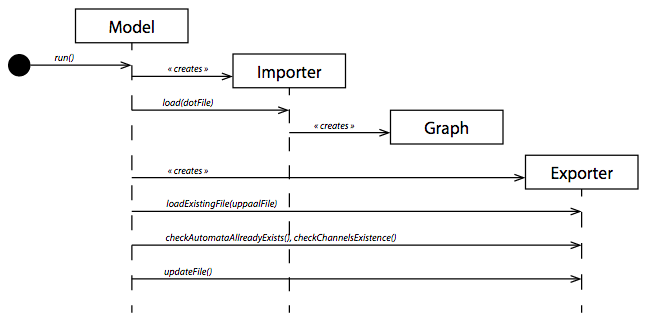
\includegraphics[scale=0.6]{ressources/deroulement.png}
  \caption{Schéma du déroulement du programme (non formalisé)}
\end{figure}

La ressource la plus importante est le graphe car il est généré par l'importeur 
puis utilisé par l'exporteur -- non représenté mais passé à la création -- pour 
vérifier la compatibilité avec le projet UPPAAL et la conversion dans le bon format.
\\\\
Par ailleurs, au niveau de l'implémentation -- avec l'interface graphique -- nous 
avons découpé cette routine en étapes. Ceci nous a permis de pouvoir reprendre 
à n'importe quel moment si il y a eu un souci et que l'utilisateur est en moyen de 
le résoudre via l'interface.
\\\\

\section{Choix techniques}
\subsection*{Technologie}
Nous avons décidé d'utiliser la technologie JAVA pour développer notre 
solution car elle a été utilisé par les développeurs du projet \textsc{Uppaal}.
\\\\
\textsc{Uppaal} n'est pas open source mais s'il le devient ce sera alors plus facile d'intégrer
notre solution d'import directement en interne.

\subsection*{Aspect mis de coté}
Afin de nous concentrer sur la conversion du graphe et l'importation dans le projet \textsc{Uppaal},
le logiciel ne prend pas en compte la disposition graphique des éléments de l'automate.
\\\\
Il se contente alors de les afficher en ligne afin de pouvoir les identifier facilement mais 
l'utilisateur devra les réorganiser lui-même sachant que \textsc{Uppaal} n'intègre pas de fonctions de 
réorganisation automatique

\section{Documentation du module Hetersys}
\subsection{Liste des fonctionnalités}
Afin d'aider à mieux appréhender le module et comprendre ce qu'il est capable ou non de faire voici
une liste de ces fonctionnalités (datée du \textit{7 avril 2015}).

\subsubsection*{Importation et exportation}
\begin{itemize}
	\item Importation d'un automate décrit au format DOT
	\item Listing des canaux utilisés par l'automate à intégrer	
	\item Chargement d'un système décrit sous forme de projet \textsc{Uppaal}
	\item Listing des automates du système
	\item Listing des canaux déclarés dans le système
	\item Intégration de l'automate dans le système
\end{itemize}

\subsubsection*{Vérifications et intégration}\label{ssec:VerifList}
\begin{itemize}
	\item Automate en doublon entre celui à ajouter et ceux dans le système (suivant le nom)
	\item Présence d'au moins un canal utilisé par l'automate (à intégrer) déclaré dans le système
	\item Ajout des canaux utilisés par le nouvel automate dans le système (au cas par cas)
\end{itemize}

\subsection{Fenêtre principale}

Il s'agit du premier élément auquel l'utilisateur est confronté mais l'interface a été 
pensée pour faciliter l'apprentissage.

\begin{figure}[!h]
  \centering
  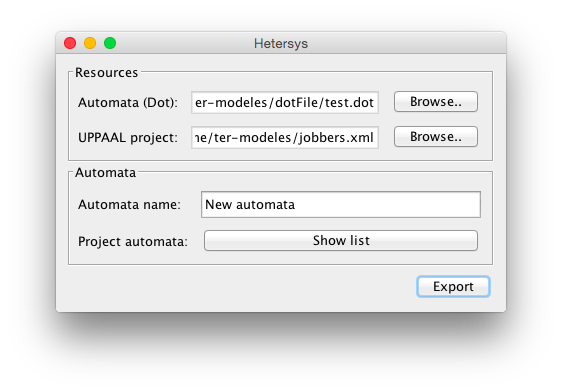
\includegraphics[scale=0.6]{ressources/gui/home.png}
  \caption{Fenêtre principale}
\end{figure}

En effet elle est décomposée en 2 parties: \emph{Resources} et \emph{Automata}. 
\\\\
La première partie regroupe les fichiers dont le programme à besoin en entrée à savoir 
un automate -- décrit sous forme de graphe en DOT -- et un projet \textsc{Uppaal} pré-existant.
\\\\
La seconde section s'intéresse à l'automate qui sera ajouté dans le projet. Dans un projet
\textsc{Uppaal}, chaque automate a un nom pour pouvoir l'identifier de manière unique ce qui veut
dire que deux automates ne peuvent pas avoir le même nom. C'est pourquoi le bouton 
\og{}Show list\fg{} permet d'afficher le nom des automates déjà présents dans le projet 
afin de ne pas les réutiliser.
\\\\
Un appui sur le bouton export permet simplement d'exporter l'automate -- au format DOT -- 
dans le projet \textsc{Uppaal} donné.

\subsection{Gestion des canaux}

L'automate donné en entrée n'ayant pas de contraintes particulières -- si ce n'est respecter 
le format DOT -- il n'est pas obligatoire que celui-ci ait des canaux en commun avec 
les autres automates du projet.
\\\\
C'est pourquoi, notre module va se charger de scanner les canaux utilisés dans l'automate 
et dans le projet pour notifier l'utilisateur dans 2 cas particuliers.

\subsubsection*{Canaux non déclarés}

Dans le cas où l'automate en entrée utiliserait des canaux qui ne sont pas déclarés
dans le projet \textsc{Uppaal}, notre module demandera à l'utilisateur s'il veux les 
importer.

\begin{figure}[h]
  \centering
  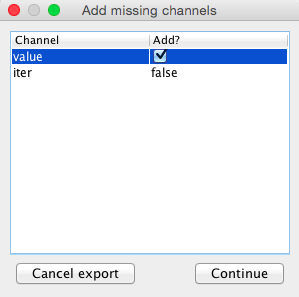
\includegraphics[scale=0.6]{ressources/gui/channels.png}
  \caption{Ajout de canaux}
\end{figure}

La liste des canaux permet de décider au cas par cas quel canaux il faut importer ou pas.

\subsubsection*{Aucun canal en commun}
Le but de ce logiciel étant de composer les automates entre eux, lorsque l'automate en 
entrée n'a aucun canal en commun avec ceux dans le projet un message d'alerte apparaît.

\begin{figure}[h]
  \centering
  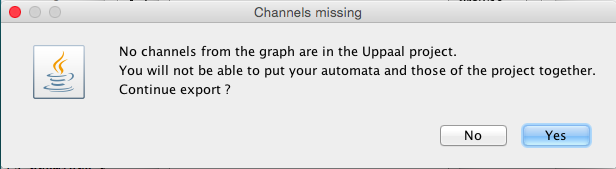
\includegraphics[scale=0.6]{ressources/gui/missing.png}
  \caption{Aucun lien entre les automates}
\end{figure}

Ceci permet à l'utilisateur d'annuler l'export pour changer son automate et utiliser 
des canaux déjà existants avant de le ré-exporter.

\subsection{Messages d'information}
\subsubsection*{Automate en double}
L'automate à insérer ne doit pas porter le même nom que ceux déjà dans le projet donc
une fenêtre notifie l'utilisateur si c'est le cas.

\begin{figure}[h]
  \centering
  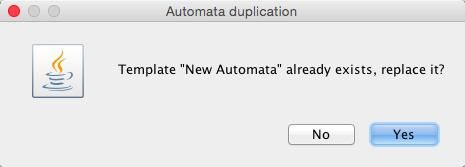
\includegraphics[scale=0.6]{ressources/gui/exists.png}
  \caption{Automate en double}
\end{figure}

\subsubsection*{Fin de l'export}
L'export d'un automate est très rapide mais le logiciel notifie quand même 
l'utilisateur quand celui-ci est terminé. 

\begin{figure}[h]
  \centering
  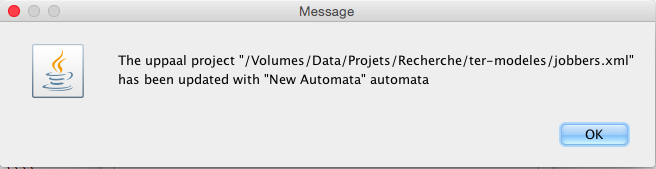
\includegraphics[scale=0.6]{ressources/gui/success.png}
  \caption{Export réussi}
\end{figure}

Le message rappelle quel projet \textsc{Uppaal} a été modifié pendant l'opération mais 
aussi le nom de l'automate qui a été ajouté.

\chapter{Expérimentations et validation}

    Afin d'expliciter les résultats obtenus grâce à notre application, nous allons 
    prendre deux cas concrets. Nous pourrons alors voir à travers eux les extensions 
    possibles de notre programme.
    
    \section{Cas du robot travailleur}
    
    Notre premier exemple est le cas qui à servi d'exemple précédemment : le robot travailleur.
    Le principe est basique, un travailleur se sert d'outil (un marteau et un maillet) 
    pour usiner des objets.
\\\\
    Pour commencer, nous avons créé le cas le plus simple sous \textsc{Uppaal} : un travailleur, 
    travaillant sur un seul objet. Pour travailler sur cet objet, il peut se servir 
    d'un maillet ou d'un marteau, cependant pour le moment il n'a qu'un marteau à sa 
    disposition.

\begin{figure}[H]
  \centering
  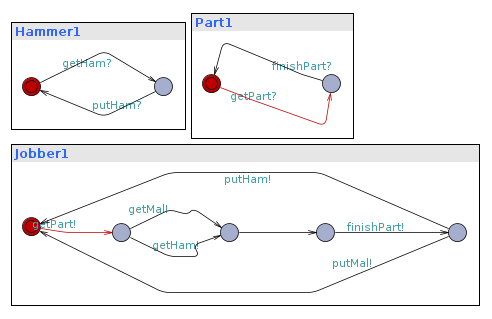
\includegraphics[scale=0.6]{ressources/workerBasic.png}
  \caption{Cas de départ}
\end{figure}

    Le fonctionnement est plutôt simple, le robot travailleur commence par prendre un objet, puis un outil disponible. Une fois qu'il a fini de travailler, il pose son outil, puis l'objet.
\\\\
    Pour enrichir notre système, on souhaite ajouter la possibilité au travailleur de prendre l'outil mallet. Pour ce faire on commence par créer un fichier dot, décrivant le fonctionnement du mallet, puis on lance notre application pour l'ajouter au système déjà existant.
    
\begin{figure}[H]
  \centering
  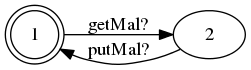
\includegraphics[scale=0.6]{ressources/mallet.png}
  \caption{L'automate maillet}
\end{figure}    

    L'ajout du maillet au système, ne nécessite pas la création de nouveau canaux, car 
    il utilise ceux déjà existant. Après la simulation dans \textsc{Uppaal}, on constate 
    que l'automate maillet est parfaitement intégré, le travailleur prenant
     aléatoirement le marteau ou le maillet pour travailler.

\begin{figure}[H]
  \centering
  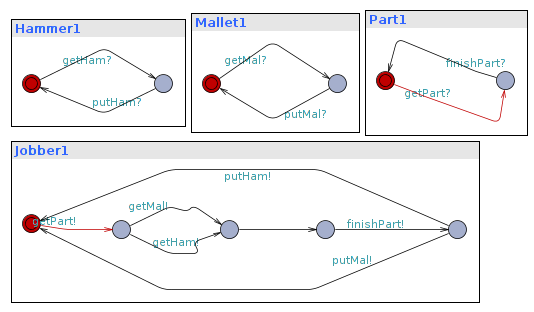
\includegraphics[scale=0.6]{ressources/workerMallet.png}
  \caption{Cas après l'ajout de l'automate maillet}
\end{figure}  

\newpage    
    \section{Cas de la surveillance caméra-écran}

    Pour illustrer le fonctionnement de notre programme, nous avons choisi un second 
    exemple, celui d'un système de surveillance. Cet exemple est un des cas sur lesquels l'équipe 
    AeLoS travaille : une caméra de surveillance filme une pièce et envoie en continue 
    les images à un écran qui les affiche.
    
\begin{figure}[H]
  \centering
  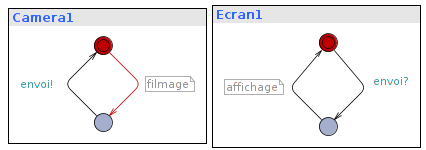
\includegraphics[scale=0.6]{ressources/cameraBasic.png}
  \caption{Cas de départ}
\end{figure}       

    Maintenant, nous souhaitons rajouter une fonction de sauvegarde à notre système. 
    Avant que les images ne soit affichées sur un écran elle doivent être enregistrées. 
    L'automate représentant ce comportement est assez simple : il récupère la vidéo de la 
    caméra, l'enregistre et la renvoie ensuite à l'écran.

\begin{figure}[H]
  \centering
  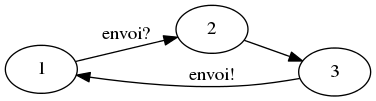
\includegraphics[scale=0.6]{ressources/save.png}
  \caption{L'automate de sauvegarde}
\end{figure} 

\newpage
    L'automate est intégré au système. Cependant le fonctionnement n'est pas celui attendu. En effet, nous souhaitions que systématiquement l'enregistrement passe par la caméra, ce qui n'est pas le cas ici. Lors de l'envoi de l'image par la caméra, la réception sera faite aléatoirement par ceux qui attendent cette enregistrement : le système de sauvegarde ou l'écran.
    
\begin{figure}[H]
  \centering
  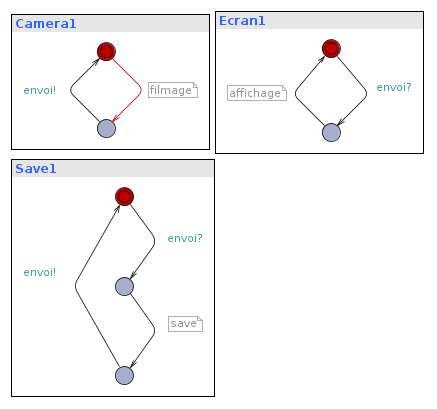
\includegraphics[scale=0.6]{ressources/cameraSave.png}
  \caption{Cas après l'ajout de la fonction de sauvegarde}
\end{figure}     
    
    Afin d'obtenir le comportement obtenu, il faudrait empêcher la communication caméra/écran. On pourrait par exemple, créer un canal spécifique entre la sauvegarde et l'écran. De cette manière, la communication se fera toujours comme souhaitée.

\newpage
\section{Problèmes connus}
Cette partie expose les soucis que peut engendrer notre solution.
\\\
En effet, quand l'on ajoute un nouvel automate dans un projet \textsc{Uppaal} et que l'on 
veut lancer une simulation ce n'est pas possible.

Ceci est lié au fait que pour tout automate présent dans le projet, \textsc{Uppaal} oblige à 
avoir une "instance" dans le système. Cependant, nous considérons que notre logiciel doit 
seulement se soucier de la cohérence entre les modèles et non de leur utilisation : c'est 
donc de la responsabilité de l'utilisateur.

\section{Conclusion}
    Nous avons conscience des limites de notre application, cependant nous nous sommes concentrés sur l'ajout d'un automate à un système existant.
\\\\
    L'intégration (avec compatibilité) dans le système existant est le cœur du sujet de 
    recherche qui en est pour l'instant à ces débuts. Cependant, notre solution intègre déjà les vérifications suivantes :
    
    \begin{itemize}
    \item Existence d'un automate du même nom,
    \item Indication des canaux communs entre l'automate à insérer et le projet \textsc{Uppaal},
    \item Ajout à la demande des nouveaux canaux pendant l'insertion.
    \end{itemize}
    
Pour conclure, le but premier de notre outil -- qui est rempli --  est d'insérer un automate 
dans un projet \textsc{Uppaal} mais dans le futur ce sera la partie 
\emph{gestion de la cohérence} qui sera prédominante car il s'agit du sujet de recherche.


\chapter{Bilan}
\section{Résultats}
Après avoir étudié les 3 solutions proposées par l'équipe AeLoS (section \ref{sec:Solutions}) pour composer des systèmes hétérogènes, 
nous avons choisi de nous concentrer sur la première qui repose sur le principe d'adaptation.
\\\\
En effet, pour faire communiquer 2 automates de nature différente on peut essayer d'en modifier un 
pour qu'il s'adapte -- dans sa forme -- au second. Nous avons donc implémenté une solution reposant sur 
le logiciel \textsc{Uppaal} qui lui propose de composer des automates entre eux.
\\\\
Notre solution -- appelée Hetersys -- permet d'importer un automate décrit sous forme de graphe -- au format DOT --
dans un projet \textsc{Uppaal} qui contient d'autres automates. L'adaptation de l'automate se fait donc de manière naturelle
-- par le passage au format graphe -- et ce car n'importe quel type d'automate peut être représenté sous cette forme.

\section{Perspectives}
La solution que nous avons implémentée constitue un noyau d'application -- fonctionnel de bout en bout -- qui a été conçu 
pour être facilement extensible pour les personnes qui voudront y ajouter des fonctionnalités. 
\\\\
Nous nous sommes concentrés sur
le langage DOT pour représenter les graphes -- pour accélérer le développement -- mais il serait intéressant de pouvoir définir des types de syntaxes.
Cela permettrait aux langages dont la syntaxe est proche de ne pas avoir à redéfinir un importeur dont juste les mots (ou les symboles)
liés au langage seraient changés. 
\\\\
Si l'on se ressitue au niveau du problème dans sa globalité, notre outil permet de gérer l'ajout de composants logiciels
dans un système hétérogène mais il n'intègre pas encore tous les éléments liés à cette opération. 
\\\\
Cela s'explique par le fait que la recherche sur le sujet n'est pas finie, elle demande donc plus de travail pour identifier
les points qui doivent être vérifiés lors de l'ajout -- ou de la suppression -- d'un modèle au sein d'un système hétérogène.
\\\\
Notre travail peut tout de même constituer une base pour tester des hypothèses sur le sujet et éventuellement  -- au travers
d'évolutions -- être un support pour démontrer par des expérimentations les résultats de la recherche.

\bibliographystyle{plain}
\bibliography{biblio}

\end{document}
